\section{Les Bases}

\subsection{Le jeu}
Afin de pouvoir modéliser correctement le jeu, il faut au préalable fixer les règles du jeu :
\begin{itemize}
    \item Il y a 24 tuiles différentes, pour un total de 72.
    \item Il y a 4 structures différentes (champ, ville, route, abbaye).
    \item Il y a 7 pions par joueur.
    \item Chaque joueur pioche et joue une tuile.
    \item Si un joueur ne peut pas poser la tuile, il passe son tour et la tuile est défaussée.
    \item Chaque joueur peut choisir de placer un de ses pions sur la tuile.
    \item Les pions ne sont récupérés que quand la structure (route, ville, champ et abbaye) est finie.
\end{itemize} 

\vspace{0.5cm}

\smallbreak
\underline{\textbf{Début de la partie}} \\
\indent Au début, on dispose de la carte de départ dans la table. Ensuite, il faut mélanger les tuiles. Chaque joueur reçoit 7 partisans (pions) correspondant à la couleur de son choix.\\
La phase d'initialisation prépare le plateau afin qu'il soit fonctionnel :
\begin{itemize}
    \item Création du plateau
    \item Configuration des joueurs
    \item Création et mélange du deck
\end{itemize}

\smallbreak
\underline{\textbf{La boucle de jeu}}

\indent On peut schématiser un tour de jeu comme suit :

\hspace{-1.5cm}


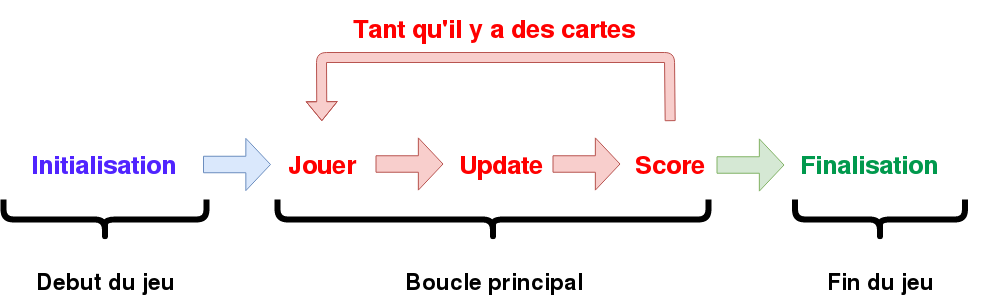
\includegraphics[scale=0.5]{Schema.png}
\hspace{1.5cm}


\vspace{0.5cm}

Les joueurs jouent à tour de rôle tant qu'il y a des tuiles à piocher. A chaque tour, ils doivent réaliser les actions suivantes en respecter l'ordre indiqué également : 
\begin{itemize}
    \item Un joueur pioche une tuile
    \item Il joue cette tuile
    \item Il place son pion
    \item Il gagne des points
\end{itemize}

\noindent Si grâce à cette tuile, il réussit à achever des chemins, des villes ou des abbayes, tous les joueurs doivent les évaluer et compter les points correspondants.
Et enfin, lorsqu'il n'y a plus de tuiles à piocher,  on compte les points restant pour départager les joueurs.

\subsection{Les impératifs}
La modélisation de ce jeu requiert différents points. Tout d'abord, il faut trouver une représentation propice des différents composantes : comment choisir les structures des tuiles et du plateau de jeu ? Comment modéliser les villes, champs, routes et abbayes ? Ensuite, il faut conceptualiser les algorithmes gérant la dynamique du jeu pour qu'ils collent au fonctionnement attendu. De plus, il faut répartir ces fonctions dans plusieurs fichiers sources, et donc trouver un découpage adéquat. Enfin, pour gérer la compilation séparée de ces fichiers et ne pas recompiler inutilement des fichiers non modifiés, il faut établir un Makefile gérant les compilations.
\subsection{Choix d'implémentation}

La particularité de "Carcassonne" est que le plateau de jeu n'est pas fixe. On part d'un plateau vide qui devient plus grand à chaque tour de jeu .
De plus, les tuiles du jeu contiennent pleins d'informations, d'où les différentes structures.
\subsubsection{Une tuile}

Une tuile est modélisée par une structure \textit{tuille} qui contient les champs suivant : 
\begin{itemize}
\item \textbf{type} : Un tableau d'entiers $(4\times3)$ qui contient le type du milieu en fonction de sa position $NORTH$, $WEST$, $SOUTH$ et $EAST$.
\item \textbf{dir} : Une énumération de direction décrivant l'orientation de la tuile.
\item \textbf{milieu} : Un entier représentant le type du milieu au centre de la tuile (important pour les carrefours et les villes).
\item \textbf{shield} : Un booléen mentionnant si la ville contient un bouclier.
\item \textbf{position} : Un tableau contenant deux champs $(x,y)$ représentant position de la tuile sur le plateau.
\item \textbf{pion} : Un tableau $(4\times3)$ qui indique s'il y a un pion sur l'une des cases de la tuile et qui en est le propriétaire.
\item \textbf{id} : Un $id$, propre au type de la tuile.
\end{itemize}

\vspace{0.5cm}

Les tuiles sont initialisées comme ceci: une tuile fantôme "NULL" . 
\begin{verbatim}
struct tuille {
  int type[4][3] = {{ NONE, NONE, NONE}, {NONE, NONE, NONE}, 
  {NONE, NONE, NONE}, {NONE, NONE, NONE}};
  enum direction dir = NORTH;
  int milieu = NONE ;
  int shield = NONE;
  int position[2] = {NONE,NONE} ;
  int pion[4][3] = {{ NONE, NONE, NONE}, {NONE, NONE, NONE}, 
  {NONE, NONE, NONE}, {NONE, NONE, NONE}};
  int id = NONE;
};
\end{verbatim}


Voilà un exemple de tuile:  

\begin{verbatim}
struct tuille {
  int type[4][3] = {{ 1, 1, 1}, {0, 2, 0}, {0, 0, 0}, {0, 2, 0}};
  enum direction dir = NORTH;
  int milieu = 2 ;
  int shield = FALSE;
  int position[2] = {NONE,NONE}; #initialisation
  int pion[4][3] = {{ 0, 0, 0}, {0, 0, 0}, {0, 0, 0}, {0, 0, 0}};
  int id_img = 7;
};
\end{verbatim}

Elle correspond à la tuile :\\

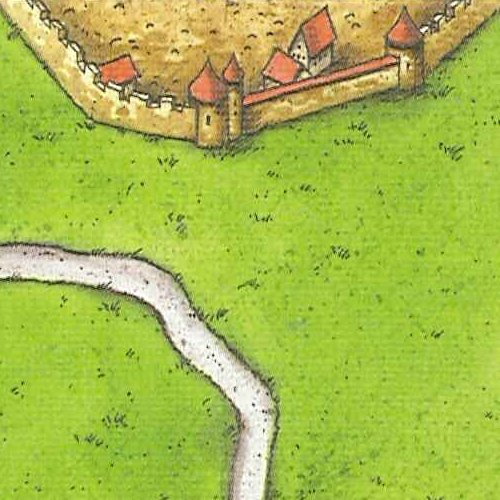
\includegraphics{card07.jpg} 
\hspace{2cm}
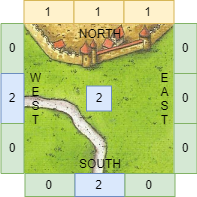
\includegraphics[scale = 0.5]{StructTuile2.png}
\newline 
    
La tuile suivante montre l'importance du choix du champ \textbf{milieu} dans la structure \textbf{tuille} : savoir si les bords de la tuile passent par le milieu ou s'il s'agit de deux zones distinctes. Par exemple, sans ce champ, on ne peut pas faire la différence entre ces deux tuiles :
\newline
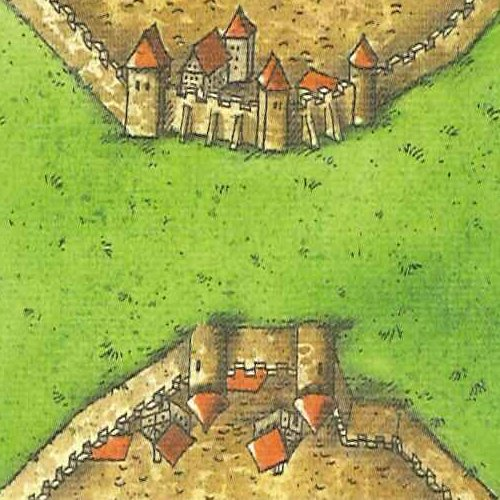
\includegraphics{card05.jpg}
\hspace{3cm}
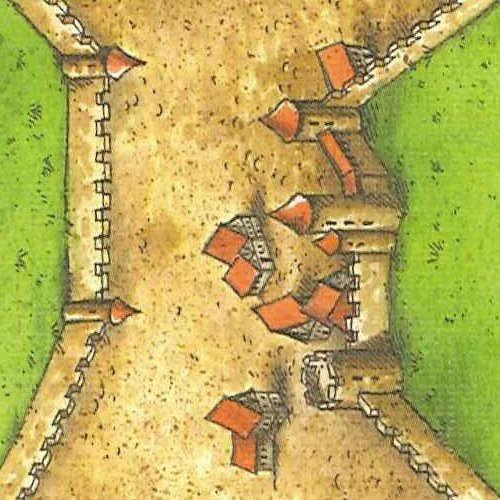
\includegraphics{card09.jpg}


Afin de faciliter le comptage des points et le positionnement des pions, un chemin, un champ, une abbaye et une ville sont chacune modélises par une structure. En effet, si on stocke dans des structures l'avancement de ces  différents édifices, il est possible de connaître leur statut (fini ou non), et ce, sans faire des parcours. A condition qu'elles soient mises à jour à chaque tour de jeu.

\vspace{0.5cm}

\noindent Pour faciliter leur utilisation, des structures supplémentaires ont été définies :

\vspace{0.5cm}

\noindent \textbf{link} : une structure de liste doublement chaînée (avant et arrière) avec un pointeur en tête et en queue, avec une donnée quelconque. 
\begin{verbatim}
struct link {
  struct lelement * head; 
  struct lelement * tail;
  int taille; 
};
\end{verbatim}

  \noindent\textbf{lelement} : une structure d'élément contenant une donnée quelconque et deux pointeurs vers l'élément suivant et précèdent .

\begin{verbatim}
struct lelement {
  void * data; 
  struct lelement * next; 
  struct lelement * previous;
};
\end{verbatim}


\begin{center}
   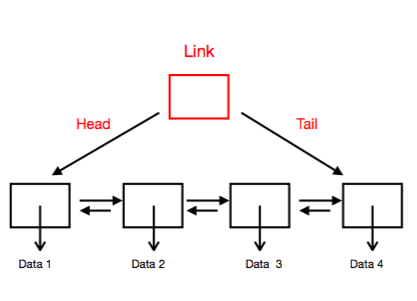
\includegraphics[scale=0.6]{liste_chainee.png} 
\end{center}


\noindent\textbf{triplet} : afin d'éviter les conflits entre les édifices lors de la recherche sur le plateau de jeu. 

\begin{verbatim}
struct triplet{
  int x; 
  int y;
  int z;
};
\end{verbatim}

L'exemple de tuile suivante montre bien que sans cette information supplémentaire, on ne peut pas faire de distinction entre les différentes routes :


\begin{center}
   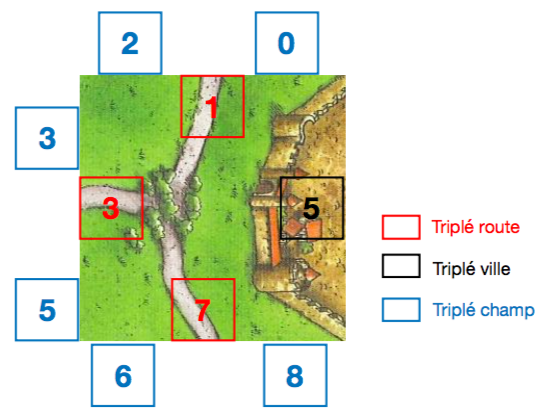
\includegraphics[scale=0.5]{tutuile.png} 
\end{center}


\subsubsection{Une route}

Une route est modélisée par une structure 
 \textbf{route} mise à jour à chaque fois qu'une tuile est ajoutée sur le plateau de jeu. Elle contient les champs suivants :


\begin{itemize}
    \item \textbf{lst\_tutuile} : la liste des tuiles qui la composent.
    \item \textbf{lst\_triplet} : la liste des triplets qui la composent.
    \item \textbf{voleurs} : les pions que chaque joueurs possède sur la route.
    \item \textbf{avancement} : l'état de la route (0 pas d'extrémité, 1 une extrémité, 2 la route est finie).
    \item \textbf{len} : taille de la liste des tuiles.
    
    
\end{itemize}


\begin{verbatim}
struct road {
  struct link * lst_tutuille; 
  struct link * lst_triplet; 
  struct link * lst_champ;
  int voleurs[PLAYER_MAX];
  int avencement;
  int len;
};
\end{verbatim}



Exemple d'une \textit{struct road} : 

\begin{verbatim}
struct road {
  struct link * lst_tuile = lnk -> T1 <-> T2 <-> T3 <-> T4 
  # la liste des tuiles
  struct link * lst_triplet = lnk -> {0,0,7} <-> {1,0,5} <-> {1,0,7} etc.
  #la liste des triplets
  int voleurs[PLAYER_MAX] = {1, 1, 0} 
  # seul le joueur 3 n'a pas de voleur sur la route
  int avencement = 1
  # la route a déjà une extrémité : la tuile1
  int len = 4 
  # ce qui fait 4 points pour les joueurs 1 et 2
};
\end{verbatim}

\newpage
Elle correspond à la route: 

\vspace{0.5cm}

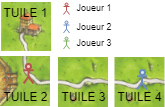
\includegraphics[scale = 1.5]{RoadEx.png}

\vspace{1cm}

\subsubsection{Un champ}

Un champ est représenté par une structure \textbf{field} 
 qui est mise à jour après chaque ajout de tuile sur le plateau de jeu. Cette structure n'est pas utilisée en elle-même. Elle est présente pour compléter la structure ville et simplifier le comptage des points. Elle contient les champs :

\begin{itemize}
    \item \textbf{lst\_tutuille} : la liste des tuiles qui la composent.
    \item \textbf{lst\_triplet} : la liste des triplés qui la composent. 
    \item \textbf{paysans} : un tableau qui indique le nombre de paysans que chaque joueur possède sur le champ.
    \item \textbf{len} : la taille de la liste.
    \item \textbf{intown} : un booléen qui indique si le champ appartient à une ville.
\end{itemize} 

\begin{verbatim}
struct field {
  struct link * lst_tutuille; 
  struct link * lst_triplet;
  int paysans[PLAYER_MAX]; 
  int len; 
  int inTown;
};
\end{verbatim}


\newpage

Exemples de \textit{struct field} : 

\vspace{0.5cm}

\begin{verbatim}
struct field A {
  struct link * lst_tutuille -> T1 <-> T2 <-> T3 <-> T4 <-> T5 <-> T6
  struct link * lst_triplet -> {0,0,8} <-> {0,0,9} <-> {0,0,10} etc
  int paysans[PLAYER_MAX] = {2, 1, 0}
  int len = 6
  int inTown = 1
};
\end{verbatim}

\begin{verbatim}
struct field B{
  struct link * lst_tutuille -> T1 <-> T4 <-> T5 <-> T6 
  struct link * lst_triplet -> {0,0,2} <-> {0,0,3} <-> {0,0,4} etc
  int paysans[PLAYER_MAX] ={0, 1, 1}
  int len = 4
  int inTown = 1
};
\end{verbatim}

Ce qui correspond à : 

\vspace{0.5cm}

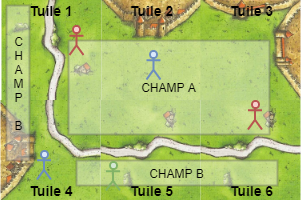
\includegraphics[scale = 0.7]{FieldEx.png}

\subsubsection{Une ville}

Une ville est représentée par une $structure$ $city$  qui est mise à jour après chaque ajout de tuile sur le plateau. Cette structure contient aussi la liste des champs qui l'entourent afin de simplifier le calcul des points liés aux champs en fin de partie. Elle contient les champs :  

\vspace{0.5cm}

\begin{itemize}
    \item \textbf{lst\_tutuille} : la liste des tuiles qui composent la ville
    \item \textbf{lst\_champ} : la liste des champs  adjacents à la ville
    \item \textbf{lst\_triplet} : la liste des triplés qui composent la ville
    \item \textbf{chevaliers} : un tableau qui indique le nombre de chevaliers que chaque joueur possède dans la ville
    \item \textbf{border} : le nombre de bord non fini de la ville (0 = ville finie)
    \item \textbf{len} : la taille de la ville 
    \item \textbf{shield} : le nombre de boucliers \newline
\end{itemize}  

   
\begin{verbatim}
struct city {
  struct link * lst_tutuille; 
  struct link * lst_champ; 
  struct link * lst_triplet;
  int chevaliers[PLAYER_MAX]; 
  int border; 
  int len; 
  int shield;
};
\end{verbatim}
 
\vspace{0.5cm}

Exemple d'une \textit{struct city} :

\begin{verbatim}
struct city {
  struct link * lst_tutuille-> T1 <-> T2 <-> T3 <-> T4 <-> T5 <-> T6 
  <-> T7 <-> T8 <-> T9
  struct link * lst_champ -> CA <-> CB <-> CC
  int paysans[PLAYER_MAX] = {1, 0, 2}
  int fini = FALSE
  int shields = 1
  int len = 5
};
\end{verbatim}

\newpage

Ce qui correspond à : 

\vspace{0.5cm}

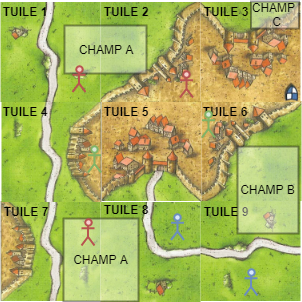
\includegraphics[scale = 0.5]{TownEx.png}

\subsubsection{Une abbaye}

Une abbaye est représentée par une structure \textit{abbaye}. Elle contient les champs :

\begin{itemize}
    \item \textbf{cloister} :la tuile qui représente l'abbaye
    \item \textbf{voisin} :le nombre de tuiles voisines
    \item \textbf{possesseur} :le joueur qui possède l'abbaye \newline
\end{itemize}  
\begin{verbatim}
struct abbaye {
  struct tuille cloister;
  int voisin;
  int possesseur;
};
\end{verbatim}

\subsubsection{Le plateau de jeu}

Enfin le plateau de jeu est modélisé par une structure $structure$ $boardgame$ qui contient les champs :

\begin{itemize}
    \item \textbf{board} :le tableau de jeu
    \item \textbf{fields} :la liste des champs
    \item \textbf{roads} :la liste des routes
    \item \textbf{cities}: la liste des villes
    \item \textbf{deck}:le deck des cartes (tuiles)
    \item \textbf{abbayes} :la liste des abbayes
  \item \textbf{points} : les points de chaque joueur 

\end{itemize}

\begin{verbatim}
struct boardgame {
  struct tuille board[2*CARD_MAX+1][2*CARD_MAX+1]; 
  struct link * fields;
  struct link * roads; 
  struct link * cities; 
  struct tuille deck[CARD_MAX]; 
  struct link * abbayes; 
  int points[PLAYER_MAX];
};
\end{verbatim}

\indent  Le plateau de jeu est représenté sous la forme d'un tableau de taille $2CARD\_MAX\times 2CARD\_MAX+1$ pour pouvoir avoir accès en temps constant aux cases adjacentes au détriment de la complexité mémoire.